\section{F25 results and discussion}
\label{sec:f25_results}

All 22 optimizations completed their 100 proposals with five runs each, and all
85 configurations were trained with the 20 reporting seeds, giving 11,000
tuning runs and 1,700 reported runs. Every confusion matrix contains 100 test
passages per scenario. All reported accuracies were recomputed from the stored
confusion matrices, and the selected hyperparameters were checked against the
optimization databases. The simulations were run in MATLAB R2021a, and the
networks were trained on an NVIDIA GeForce RTX 2060 (6~GB) with PyTorch 2.6.0
and CUDA 11.8. The GPU driver was updated from version 591.86 to 610.88 during
the campaign, and one optimization was resumed after 65 of its 100 proposals;
the effect of the driver change was not quantified.

\subsection{Reconstruction of the source results}

Table~\ref{tab:f25_reconstruction} summarizes F25-R. The source study reports,
for each channel and input, the confusion matrix of the best of its 20
runs~\cite{fernandes2025early}; the corresponding accuracies, read from the
published figures, are therefore compared with the best of the present 20 runs
(column ``Max''). With RAW inputs, the best carbody run (71.8\%) exceeded the
published value (65.1\%), whereas the best front-bogie run (65.5\%) remained
below it (82.2\%). With PAA inputs, the best runs reached 66.6\% for the carbody
and 73.8\% for the front bogie, against the published 86.7\% and 82.1\%. The
benefit of PAA reported for the carbody sensor was reproduced in direction for
the mean (57.33\% for PAA against 49.74\% for RAW), but with a smaller
magnitude, and the best RAW run exceeded the best PAA run. On the front bogie,
PAA was the least stable configuration, with an SD of 21.30 percentage points
and three runs at 10\%.

\begin{table}[htbp]
\centering
\caption{F25-R ten-class test accuracy over 20 initialization seeds. SD is the
sample standard deviation in percentage points. The last column gives the
accuracy of the best of 20 runs in the source study, read approximately from
its published confusion matrices~\cite{fernandes2025early}.}
\label{tab:f25_reconstruction}
\small
% Generated by analyze_f25_results.py; source values are best-of-20 runs read from figures.
\begin{tabular}{llrrrr}
\toprule
Response & Input & Mean $\pm$ SD (\%) & Min (\%) & Max (\%) & Source, best run (\%) \\
\midrule
S00 & RAW & $49.74 \pm 12.86$ & 23.0 & 71.8 & 65.1 \\
S00 & PAA & $57.33 \pm 6.78$ & 41.5 & 66.6 & 86.7 \\
S01 & RAW & $49.41 \pm 11.60$ & 21.4 & 65.5 & 82.2 \\
S01 & PAA & $46.69 \pm 21.30$ & 10.0 & 73.8 & 82.1 \\
\bottomrule
\end{tabular}

\end{table}

The reconstruction gap cannot be attributed to a single cause. The crack
surrogate, the deck mesh, the software framework, the random partition, and
the optimization outcome all differ from the source
(Table~\ref{tab:f25_deviations}). The published front-bogie finalist, with a
96-unit dense layer, lies outside the reported search range, and the published
finalist architectures were not retrained. The validation objectives of the
F25-R optimizations (60.0--72.8\%) were also 8--26 percentage points higher
than the corresponding 20-run test means, a selection effect discussed in
Section~\ref{sec:f25_tuning}. The results therefore support an unresolved
reconstruction gap rather than a replication of the published accuracies.
The selected hyperparameters are listed in Table~\ref{tab:f25_hyperparameters};
the front-bogie vectors are the frozen hyperparameters of F25-X.

\begin{table}[htbp]
\centering
\caption{Hyperparameters selected by the 100-proposal searches for the F25-R
models and for the three tuned models on the carbody pitch rate (S05). Filters
are listed per convolutional layer; a superscript $p$ marks a layer followed by
max pooling.}
\label{tab:f25_hyperparameters}
\footnotesize
\setlength{\tabcolsep}{3pt}
\resizebox{\textwidth}{!}{% Generated by analyze_f25_results.py; winners of the 100-proposal searches.
\begin{tabular}{lllllrrrr}
\toprule
Study & Model & Channel & Filters & Kernels & Dense & Batch & Learning rate & Parameters \\
\midrule
F25-R & RAW-CNN & S00 & 112--48$^{p}$--112$^{p}$--48$^{p}$ & 2--5--5--4 & 48 & 40 & $9.8\times10^{-5}$ & 1,746,746 \\
F25-R & PAA-CNN & S00 & 80$^{p}$--128$^{p}$--64 & 3--5--5 & 64 & 40 & $3.2\times10^{-4}$ & 662,730 \\
F25-R & RAW-CNN & S01 & 96$^{p}$--32$^{p}$--48--96$^{p}$--32 & 2--4--5--4--5 & 64 & 32 & $5.9\times10^{-5}$ & 1,529,530 \\
F25-R & PAA-CNN & S01 & 112$^{p}$--112$^{p}$--96--32 & 2--5--3--3 & 64 & 48 & $4.9\times10^{-4}$ & 390,154 \\
F25-X tuned & RAW-CNN & S05 & 48$^{p}$--96--80$^{p}$ & 2--3--5 & 64 & 48 & $6.5\times10^{-5}$ & 7,497,738 \\
F25-X tuned & PAA-CNN & S05 & 64--80--128$^{p}$ & 3--5--3 & 48 & 32 & $8.8\times10^{-5}$ & 1,820,650 \\
F25-X tuned & PAA-MR & S05 & 32$^{p}$--64$^{p}$--32$^{p}$--80 & 2--3--3--5 & 32 & 48 & $4.7\times10^{-4}$ & 43,642 \\
\bottomrule
\end{tabular}
}
\end{table}

\subsection{Channel comparison under frozen hyperparameters}

Table~\ref{tab:f25_frozen_singles} and Fig.~\ref{fig:f25_singles}a compare the
six channels with the F25-R front-bogie hyperparameters. The carbody pitch rate
(S05) gave the highest mean in all three arms: $72.61\pm4.95\%$ for RAW-CNN,
$72.29\pm14.98\%$ for PAA-CNN, and $65.98\pm3.28\%$ for PAA-MR. The large SD of
PAA-CNN is caused by a single run at 10\%; the other 19 runs lay between 68.9\%
and 83.8\%. The vertical accelerations (S00--S02) gave intermediate results,
and the two bogie pitch rates (S06 and S07) stayed close to the 10\% chance
level in every arm. Under these frozen settings, multi-rate pooling did not
improve on the flatten-based arms.

\begin{table}[htbp]
\centering
\caption{F25-X ten-class test accuracy with frozen hyperparameters (mean
$\pm$ sample SD over 20 runs, \%). All arms use the F25-R front-bogie
hyperparameters; PAA-MR uses the PAA-CNN vector with multi-rate pooling.}
\label{tab:f25_frozen_singles}
\footnotesize
\setlength{\tabcolsep}{4pt}
\resizebox{\textwidth}{!}{% Generated by analyze_f25_results.py; percent mean +/- sample SD.
\begin{tabular}{llrrr}
\toprule
Code & Response & RAW & PAA & PAA-MR \\
\midrule
S00 & Carbody vertical & $51.10 \pm 10.47$ & $48.15 \pm 14.86$ & $22.38 \pm 1.34$ \\
S01 & Front-bogie vertical & $49.41 \pm 11.60$ & $46.69 \pm 21.30$ & $37.39 \pm 8.60$ \\
S02 & Rear-bogie vertical & $57.13 \pm 10.30$ & $51.40 \pm 20.48$ & $49.12 \pm 4.94$ \\
S05 & Carbody pitch rate & $72.61 \pm 4.95$ & $72.29 \pm 14.98$ & $65.98 \pm 3.28$ \\
S06 & Front-bogie pitch rate & $19.63 \pm 1.01$ & $15.16 \pm 4.40$ & $11.51 \pm 3.77$ \\
S07 & Rear-bogie pitch rate & $21.48 \pm 7.74$ & $13.23 \pm 4.70$ & $9.98 \pm 0.35$ \\
\bottomrule
\end{tabular}
}
\end{table}

The channel ranking has a plausible geometric explanation. The carbody pitch
responds to the difference between the vertical motions of the two bogies,
which are 16~m apart, a base comparable to the 19.95~m spans. It is therefore
sensitive to the slope of the deflected deck and to the support conditions.
This is the ``apparent profile'' mechanism through which McGeown et
al.~\cite{mcgeown2024pitch} detected pier scour from carriage pitch. The bogie
pitch, in contrast, responds to the difference between two wheelsets 2.3~m
apart, over which the long-wavelength deck deflection changes little; it is
dominated by the short-wavelength rail irregularity, which is identical in all
scenarios, and by the added noise, which scales with the standard deviation of
each signal. This interpretation is consistent with the results but was not
tested separately.

\subsection{Channel-specific tuning}
\label{sec:f25_tuning}

Channel-specific tuning changed both the accuracy and its variability
(Table~\ref{tab:f25_tuned_singles}, Fig.~\ref{fig:f25_singles}b). The highest
mean among the 18 tuned singles was obtained by PAA-MR on the carbody pitch
rate: $77.63\pm2.24\%$, with a median of 77.95\% and runs between 71.7\% and
81.1\%. Tuned PAA-CNN on the same channel reached the best single run
(88.0\%) and a similar median (77.45\%), but one run collapsed to 10\% and its
SD was 21.78 percentage points. PAA-MR/S05 has 43,642 trainable parameters,
against 1,820,650 for tuned PAA-CNN/S05 and 7,497,738 for tuned RAW-CNN/S05;
inference time and energy were not measured.

\begin{table}[htbp]
\centering
\caption{F25-X ten-class test accuracy after channel-specific tuning (mean
$\pm$ sample SD over 20 runs, \%). Each arm--channel combination has its own
100-proposal optimization.}
\label{tab:f25_tuned_singles}
\footnotesize
\setlength{\tabcolsep}{4pt}
\resizebox{\textwidth}{!}{% Generated by analyze_f25_results.py; percent mean +/- sample SD.
\begin{tabular}{llrrr}
\toprule
Code & Response & RAW & PAA & PAA-MR \\
\midrule
S00 & Carbody vertical & $60.06 \pm 8.38$ & $54.44 \pm 12.64$ & $35.73 \pm 12.90$ \\
S01 & Front-bogie vertical & $50.08 \pm 14.28$ & $70.05 \pm 8.96$ & $61.81 \pm 13.09$ \\
S02 & Rear-bogie vertical & $51.80 \pm 15.69$ & $68.61 \pm 2.52$ & $58.43 \pm 6.53$ \\
S05 & Carbody pitch rate & $70.95 \pm 14.74$ & $67.26 \pm 21.78$ & $77.63 \pm 2.24$ \\
S06 & Front-bogie pitch rate & $18.61 \pm 3.84$ & $21.62 \pm 13.13$ & $13.22 \pm 5.94$ \\
S07 & Rear-bogie pitch rate & $14.24 \pm 5.13$ & $19.35 \pm 6.32$ & $9.83 \pm 0.38$ \\
\bottomrule
\end{tabular}
}
\end{table}

\begin{figure}[htbp]
\centering
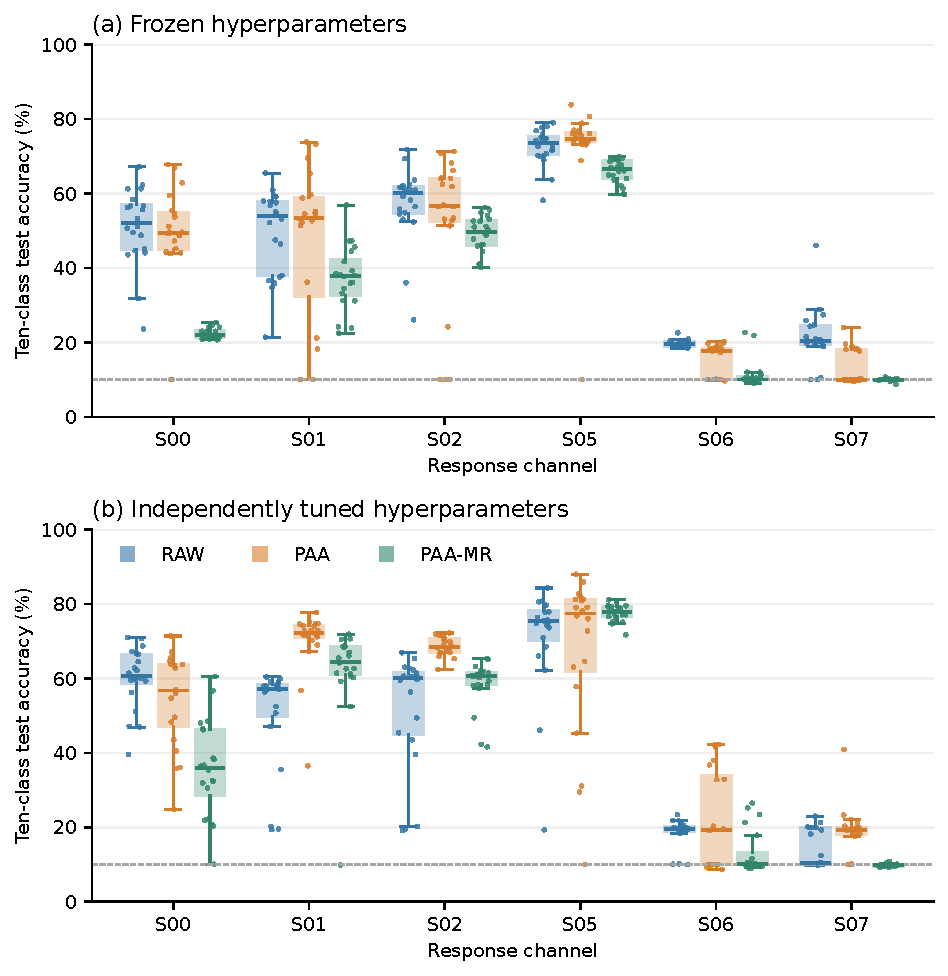
\includegraphics[width=0.92\textwidth]{f25_singles.pdf}
\caption{Distribution of the ten-class test accuracy of the six single channels
over 20 runs: (a) frozen hyperparameters; (b) channel-specific tuning. Boxes
show the median and interquartile range, whiskers extend to 1.5 times the
interquartile range, and dots show individual runs. The dashed line marks the
10\% chance level. All runs use the same passages and data partition.}
\label{fig:f25_singles}
\end{figure}

Tuning did not improve every configuration. For PAA-MR/S05, the seed-paired
gain over the frozen configuration was $+11.65$ percentage points (SD of the
paired differences 3.64), and all 20 runs improved. In contrast, the mean
accuracy of PAA-CNN/S05 decreased by 5.03 points and that of RAW-CNN/S07 by
7.25 points. Part of this behaviour is a selection effect. Each optimization
selects the best of 100 proposals on only 200 validation passages, and five
runs per proposal rarely reveal failures that occur in about one of 20
initializations. Across the 22 tuned configurations, the validation objective
of the selected proposal exceeded the subsequent 20-run test mean by 10.5
percentage points on average (range 1.4--26.1). For the S05 winners, the
validation objectives were 84.5\% (RAW-CNN), 83.5\% (PAA-CNN), and 79.4\%
(PAA-MR), against test means of 70.95\%, 67.26\%, and 77.63\%. PAA-MR/S05 thus
had the smallest optimism among the informative channels. Because all
configurations are compared on the same test set, the best configuration was
identified after the test results were known; the ranking is descriptive.

\subsection{Two-channel inputs}

Fig.~\ref{fig:f25_pairs} shows the mean accuracy of all 45 frozen pairs, and
Table~\ref{tab:f25_pairs} lists the three best pairs of each arm. All of them
contain the carbody pitch rate. A second channel rarely improved on the better
of its two members. The highest pair mean, $75.68\pm4.59\%$ for PAA-CNN with
S00+S05, exceeded the frozen PAA-CNN/S05 mean (72.29\%) only because of the
collapsed single-channel run: both medians are 74.55\%, and, paired by seed,
the pair was more accurate in only 9 of the 20 runs. For RAW-CNN, the S00+S05
pair reached $71.69\pm8.54\%$, against $72.61\pm4.95\%$ for S05 alone, and 11
of the 15 pairs had a lower mean than their better member. The only top-ranked
pair with a consistent gain was S02+S05 with PAA-MR: $70.63\pm5.16\%$, 4.65
points above PAA-MR/S05, with higher accuracy in 15 of the 20 paired runs. The
pairs were not tuned, so these comparisons concern a fixed architecture; they
are exploratory and were not used to select inputs for the regression campaign.

\begin{figure}[htbp]
\centering
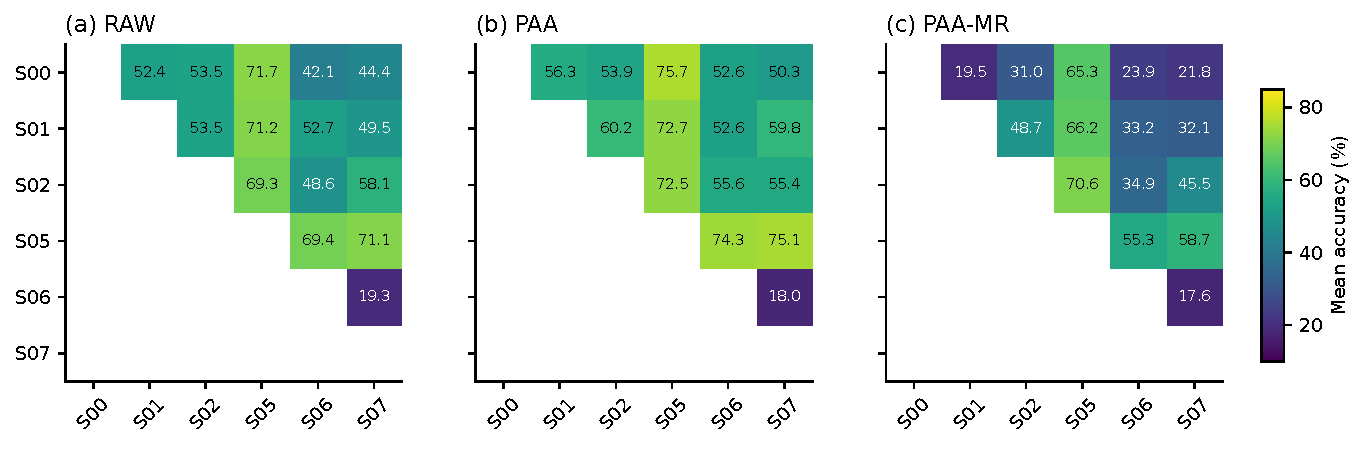
\includegraphics[width=\textwidth]{f25_pairs.pdf}
\caption{Mean ten-class test accuracy (\%) over 20 runs of the 15 two-channel
inputs with frozen hyperparameters: (a) RAW-CNN; (b) PAA-CNN; (c) PAA-MR.}
\label{fig:f25_pairs}
\end{figure}

\begin{table}[htbp]
\centering
\caption{Three best two-channel inputs of each arm with frozen hyperparameters
(ten-class test accuracy over 20 runs, \%). The ranking is exploratory.}
\label{tab:f25_pairs}
\small
% Generated by analyze_f25_results.py; exploratory test-read rankings.
\begin{tabular}{llrr}
\toprule
Arm & Response pair & Mean $\pm$ SD (\%) & Median (\%) \\
\midrule
RAW & S00+S05 & $71.69 \pm 8.54$ & 73.10 \\
RAW & S01+S05 & $71.20 \pm 6.83$ & 73.45 \\
RAW & S05+S07 & $71.12 \pm 5.36$ & 72.90 \\
PAA & S00+S05 & $75.68 \pm 4.59$ & 74.55 \\
PAA & S05+S07 & $75.08 \pm 3.60$ & 75.30 \\
PAA & S05+S06 & $74.28 \pm 6.40$ & 73.75 \\
PAA-MR & S02+S05 & $70.63 \pm 5.16$ & 71.65 \\
PAA-MR & S01+S05 & $66.17 \pm 10.69$ & 67.40 \\
PAA-MR & S00+S05 & $65.33 \pm 7.09$ & 67.75 \\
\bottomrule
\end{tabular}

\end{table}

\subsection{Discrimination of damage types}

For tuned PAA-MR/S05, the mean accuracies of the three damage coordinates were
99.97\% for the bearing condition, 97.63\% for the scour level, and 77.76\% for
the crack label. The corresponding majority-class rates are 60\%, 40\%, and
50\%, because the catalogue is not balanced along each coordinate. Bearing
damage and scour level were thus recognized almost perfectly from a single
carbody channel, and the crack label limited the overall accuracy.

The mean confusion matrix (Fig.~\ref{fig:f25_confusion}) shows this structure
directly. All eight off-diagonal entries above 10\% involve pairs of scenarios
that differ only in the crack coordinate: Healthy and DC2 (31.8\% and 24.1\%),
DC4 and DC7 (15.7\% and 14.9\%), DC5 and DC8 (19.2\% and 17.2\%), and DC9 and DC10
(37.5\% and 39.6\%). The two scenarios whose combination of scour level and
bearing condition is unique in the catalogue, DC3 and DC6, were recognized in
89.8\% and 99.1\% of the cases. The DC9/DC10 pair, which differs only in crack
severity, was also the main source of error in the published carbody results of
the source study~\cite{fernandes2025early}. Within this catalogue, a local
$EI$ reduction of 14--22\% over 0.30~m is thus much harder to recognize from the
vehicle response than a 5\% loss of support stiffness or the restraint of an
end bearing. This conclusion is conditional on the crack surrogate and its
single location.

\begin{figure}[htbp]
\centering
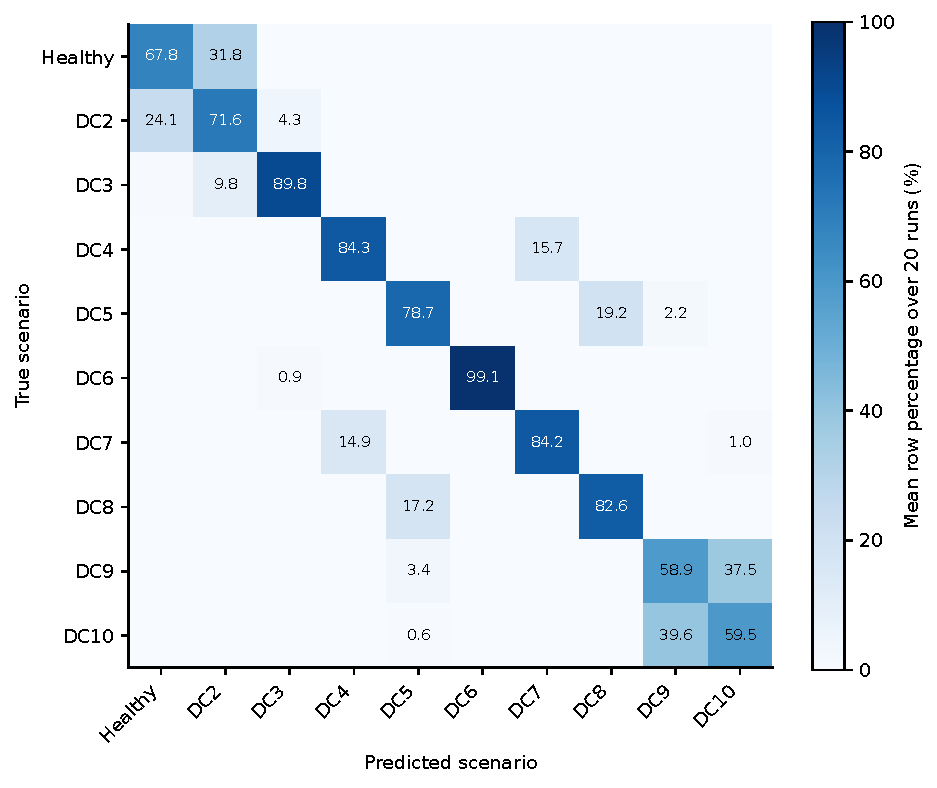
\includegraphics[width=0.82\textwidth]{f25_confusion.pdf}
\caption{Confusion matrix of tuned PAA-MR on the carbody pitch rate (S05),
averaged over the 20 runs; rows are true scenarios and entries are row
percentages. Entries below 0.5\% are not labeled.}
\label{fig:f25_confusion}
\end{figure}

\subsection{Training stability}

Of the 1,700 reported runs, 90 predicted a single class for every test passage
and 132 had an accuracy of 10\% or less. Sixty of the 90 single-class
collapses used one of the two bogie pitch rates, which are close to chance
level in any case. Excluding these single-channel configurations, single-class
collapses occurred in
26 of 500 PAA-CNN runs, 3 of 500 RAW-CNN runs, and 1 of 460 PAA-MR runs; these
counts include the two repeated F25-R control configurations. In addition, 379
runs restored a checkpoint from epoch 950 or later, 53 of them at epoch 1,000,
so the 1,000-epoch limit of the source protocol was active in part of the
runs. All runs are kept in the reported distributions. The frequency of
collapsed runs shows why a single best run, or a mean without the
distribution, is an incomplete summary of a drive-by classifier.

The F25 results concern ten fixed scenarios, one bridge, one rail profile, and
a passage-level split. They provide no evidence on continuous scour
estimation, unseen damage states, measured signals, or other rail profiles;
the four-block regression results remain pending in the next section.
